\documentclass[11pt]{beamer}
\usetheme{metropolis} % optional
\usepackage{booktabs}
\usepackage{hyperref}
\usepackage{tikz}
\usetikzlibrary{arrows.meta,positioning,shapes.geometric}

\title{Technology Diffusion}
\author{Xingxu Chai}
\institute{Frankfurt School of Finance and Management}
\date{December 3rd, 2025}

\begin{document}
\maketitle

%=================================================
% Title bite
%=================================================


\begin{frame}
\textbf{New technologies arise in every period of society.}
\begin{figure}
    \centering
    \includegraphics[width=1\linewidth]{Presentation_bootcamp/Pictures/cases.png}
\end{figure}
\end{frame}

\begin{frame}
\textbf{New technologies aren’t adopted immediately $\rightarrow$ diffusion takes time.}

\begin{figure}
    \centering
    \includegraphics[width=0.8\linewidth]{Presentation_bootcamp/Pictures/diffusion.png}
    \caption{Staggered implementation of hybrid corn; Source: Sutch, Libecap, and Steckel (2011),
updating data from Griliches (1957)}
\end{figure}
\end{frame}

\begin{frame}
\textbf{New technologies aren’t adopted immediately $\rightarrow$ diffusion takes time.}

\begin{figure}
    \centering
    \includegraphics[width=1\linewidth]{Presentation_bootcamp/Pictures/diffusion2.png}
        \caption{Different technological adoption. Source: Visual Capitalist}
\end{figure}
\end{frame}


\begin{frame}
  \vfill
  \centering
  \Large  \textbf{Why aren’t new technologies adopted immediately?}\\[1ex]
 \Large \normalsize{\textbf{Research Question(Firm-Level):}}  \textit{Why do firms adopt new technologies, and what they get in return?}

  \vfill
\end{frame}
%=================================================
% Data and Pipeline
%=================================================
%=================================================
% Data & causal graph extraction
%=================================================
%=================================================
% Literature & contribution
%=================================================

\begin{frame}{Brief overview of the literature}
\small
\begin{itemize}
\item \textbf{Technology diffusion.} Since Griliches (1957), economists have viewed diffusion as a \textbf{gradual} process (e.g.\ Mansfield, 1961, 1963; Jovanovic and Lach, 1989; David, 1990; Hall, 2006).

  \item \textbf{Drivers of diffusion.} A second strand studies which factors make diffusion faster or slower. (e.g.\ Acemoglu and Linn, 2004; Greenstone et al., 2010; Moscona, 2019).
  \begin{itemize}

  \item Usually focus on \textbf{one technology or a small set}, and measure diffusion using \textbf{physical adoption} 
        (plants, equipment...).
   \end{itemize}

  \item \textbf{Textual analysis and innovation.} Using text, recent work can capture many technologies within one measurement framework (Bloom et al., 2025). 
  \begin{itemize}

  \item By capturing \textbf{mentions} (intensity and speed). $\rightarrow$ contribute to {\color{red}"diffusion"}, not {\color{red}"drivers"}.
  \end{itemize}

\end{itemize}

\begin{itemize}
\item Most of the diffusion evidence is from macro level.
\end{itemize}
\end{frame}


\begin{frame}{What's the link to accounting literature}
\small
\begin{itemize}
  \item \textbf{Earnings calls are an important disclosure channel.} 
        Information on technology adoption discussed in earnings calls 
        is an important part of information dissemination in capital markets.

  \item \textbf{Intangible assets and measurement.}
       Many technology-related investments (software, data, AI teams, digital platforms) are expensed and remain off the balance sheet. The way managers talk about the new technologies may reveal important information about the presence and nature of these intangible assets.

  \item \textbf{Managerial learning and benchmarking.}
Managerial accounting research studies how managers benchmark against peers and learn from other firms’ management practices and technology choices.
\end{itemize}
\end{frame}



\begin{frame}{Challenge and Solution}
\small
\begin{itemize}
  \item \textbf{Hurdle.} We care about the \emph{economic meaning} of texts, 
        not just \emph{how often} a word appears (Bloom et al., 2025).  
        Traditional text tools (word counts, topic models) limit our ability 
        to uncover the reasons behind mention intensity.\\[0.3em]
        {\color{red}\textbf{Drivers of diffusion hidden in text are still a black box.}}

  \item \textbf{Solution.} Chain-of-thought LLMs make it possible to read texts 
        as causal stories. I use them to extract explicit 
        \emph{cause} $\rightarrow$ \emph{effect} statements for different 
        technologies from earnings calls.
\end{itemize}


\end{frame}






\begin{frame}{What this paper adds}
\small
\begin{itemize}
  \item I construct a new measurement to study diffusion:
    \begin{itemize}
      \item \textbf{Firm-level:} based on 450{,}486 firm-level earnings calls;

      \item \textbf{Multi-technology:} 29 disruptive technologies identified in Bloom et al.\ (2021);
      \item \textbf{Causal statements:} extract explicit \emph{cause} $\rightarrow$ \emph{effect}
            statements from these calls.
    \end{itemize}

  \item Through this process, I turn raw call text into:
    \begin{itemize}
      \item a panel of \textbf{when and where} each technology is discussed;
      \item structured measures of \textbf{why firms say they adopt}
            (causes) and \textbf{what they say happens after adoption} (effects).
    \end{itemize}


  \item In this way, the paper provides a framework that speaks to both streams of diffusion literature: 
        \emph{\textbf{What are the diffusion patterns of new technologies?}} 
        and \emph{\textbf{What forces drive these diffusion patterns?}}
\end{itemize}
\end{frame}





\begin{frame}{Methodology: From earnings calls to taxonomy}
\centering
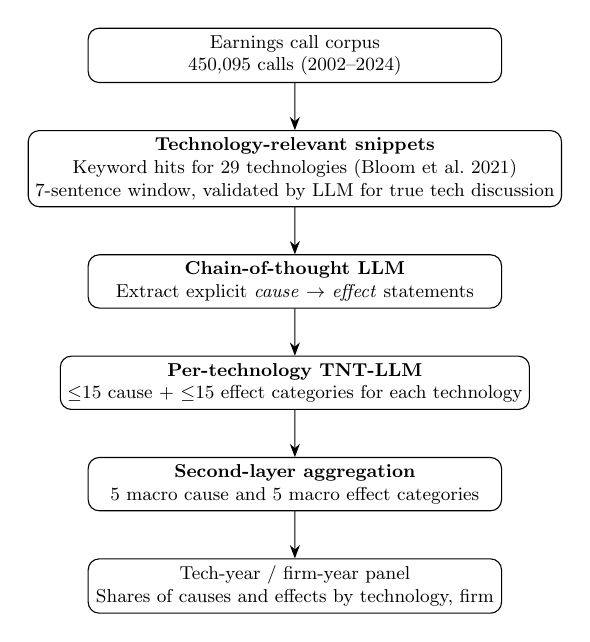
\begin{tikzpicture}[
  scale=0.75,
  every node/.style={transform shape},
  node distance=0.8cm,
  >=Stealth,
  process/.style={
    rectangle,
    rounded corners,
    draw,
    align=center,
    minimum width=7cm,
    minimum height=0.9cm,
    font=\small
  }
]

\node[process] (data) {Earnings call corpus\\
450{,}095 calls (2002--2024)};

\node[process, below=of data] (snip) {\textbf{Technology-relevant snippets}\\
Keyword hits for 29 technologies (Bloom et al.\ 2021)\\
7-sentence window, validated by LLM for true tech discussion};

\node[process, below=of snip] (cot) {\textbf{Chain-of-thought LLM}\\
Extract explicit \emph{cause} $\rightarrow$ \emph{effect} statements};

\node[process, below=of cot] (tnt) {\textbf{Per-technology TNT-LLM}\\
$\leq$15 cause + $\leq$15 effect categories for each technology};

\node[process, below=of tnt] (agg) {\textbf{Second-layer aggregation}\\
5 macro cause and 5 macro effect categories};

\node[process, below=of agg] (panel) {Tech-year / firm-year panel\\
Shares of causes and effects by technology, firm};

% Arrows
\draw[->] (data) -- (snip);
\draw[->] (snip) -- (cot);
\draw[->] (cot) -- (tnt);
\draw[->] (tnt) -- (agg);
\draw[->] (agg) -- (panel);

\end{tikzpicture}
\end{frame}



\begin{frame}{Measurement Construction——Cause-Effect Extraction}
\small
\begin{itemize}
  \item \textbf{Input.} A 7-sentence snippet from an earnings call that contains a technology keyword.
  \item \textbf{Step 1: Tech relevance.}  
        LLM checks whether the keyword filtered snippet really talks about the technology. If not, drop.
  \item \textbf{Step 2: Causal content.}  
        For relevant snippets, LLM checks \textbf{if there is a causal claim involving the technology}  
        (``leads to'', ``because of'', ``enables'', ``limits'', ``depends on'', etc.).  
        If no causal claim, stop.
  \item \textbf{Step 3: Causes and outcomes.}  
        When causality exists, LLM lists (i) explicit \textit{\textbf{upstream drivers}} of the technology and  
        (ii) explicit \textit{\textbf{downstream outcomes}} for the firm.
  \item \textbf{Step 4: Normalize into triples.}  
        LLM converts these lists into graph triples:  
        \begin{itemize}
          \item [--] [cause, \textit{promotes/suppresses}, \textbf{technology}]  
          \item [--] [\textbf{technology}, \textit{promotes/suppresses}, outcome]  
        \end{itemize}
  % \item \textbf{Step 5: Consistency check.}  
  %       LLM re-reads the snippet and drops any triple that is not clearly supported by the text,
  %       does not involve the technology, or is a tautology.
\end{itemize}
\end{frame}



\begin{frame}{Measurement Construction——Cause-Effect Extraction}
\small

\textbf{Examples of extracted triples:}

\begin{itemize}
\item Cause

\begin{itemize}

  \item open software and open hardware platforms $\rightarrow$ \textit{promotes} $\rightarrow$ Cloud computing
  \item data warehousing capabilities $\rightarrow$ \textit{promotes} $\rightarrow$ Machine Learning AI
  \item China's disengagement from US supply arrangements $\rightarrow$ \textit{suppresses} $\rightarrow$ Solar Power
\end{itemize}
\end{itemize}

 \begin{itemize}
 \item Effect
 \begin{itemize}

  \item Cloud computing $\rightarrow$ \textit{promotes} $\rightarrow$ cost effectively leverage big data at scale
  \item Machine Learning AI $\rightarrow$ \textit{promotes} $\rightarrow$ automated policy sales
  \item Solar Power $\rightarrow$ \textit{promotes} $\rightarrow$ avoids 3,000 tons of CO$_2$ emissions
\end{itemize}
\end{itemize}

\end{frame}

%=================================================
% Taxonomies (TNT-LLM)
%=================================================
\begin{frame}{Measurement Construction——Taxonomies (TNT-LLM)}
\small
\vspace{-0.5em}

\begin{itemize}
  \item After the causal statement extraction, I have about \textbf{198k} raw cause texts 
        and \textbf{385k} raw effect texts.  
        Reading them one by one is not possible.
  \item I use \textbf{TNT-LLM} to turn these raw texts into interpretable categories in three steps:
    \begin{itemize}
      \item \textbf{Creation:} Take a first small batch of texts (200 raw cause/effect phrases) for one technology and let the LLM
            propose an initial list of cause/effect categories (a draft taxonomy).
      \item \textbf{Update:} Feed more batches of texts.  
            For each batch, the LLM checks how well the current labels fit, finds gaps or overlaps,
            and refines the taxonomy (merge, split, or rename labels).
      \item \textbf{Review:} A final prompt cleans the taxonomy, checks coverage and formatting,
            and outputs a stable set of labels.
    \end{itemize}
  \item I run this loop separately for all \textbf{29 technologies}
        $\Rightarrow$ \textbf{29 technology-specific taxonomies} (category name and definition).
\end{itemize}
\end{frame}


\begin{frame}{Taxonomies by Technology (Complete in Appendix)}
\scriptsize
\begin{columns}[t]

\begin{column}{0.5\textwidth}
\textbf{Cloud Computing}\\
\emph{Causes:} \textbf{Strategic digital transformation}; Market Demand and Consumer Behavior; Investment and Funding Allocation……\\
\emph{Effects:} Revenue and Financial Growth; Scalability and Resource Management; Market Expansion and Adoption…… .\\[0.5em]

\textbf{Machine Learning / AI}\\
\emph{Causes:} \textbf{Data assets and capabilities}; Talent and Organizational Capabilities; Technology Infrastructure and Platforms……
\emph{Effects:} Personalization and Targeting; Customer Experience Enhancement;  Marketing and Advertising Optimization……
\end{column}

\begin{column}{0.5\textwidth}
\textbf{Online Streaming}\\
\emph{Causes:} \textbf{Content and Application Development}; Software and Algorithm Development; Infrastructure Deployment and Connectivity……
\emph{Effects:} Subscriber and User Growth; Revenue and Financial Performance; User Engagement and Consumption……\\[0.5em]

\textbf{Solar Power}\\
\emph{Causes:} \textbf{Government Policy and Regulation}; Economic and Cost Factors; Technological Advancements and Innovation……\\
\emph{Effects:} Cost Reduction and Efficiency; Revenue and Financial Growth; Production Capacity……
\end{column}

\end{columns}
\end{frame}


%---------------- Aggregated taxonomy: logic ----------------
\begin{frame}{Measurement Construction——Aggregated Taxonomy}
\small
\begin{itemize}
  \item After the first TNT-LLM step (run separately for each technology),  
        I end up with \textbf{293} distinct cause categories and \textbf{308} distinct effect categories
        across the 29 technologies.
  \item What are the \textbf{first-order} causes and effects across all technologies?
  \item I therefore add a \textbf{second LLM layer}:
    \begin{itemize}
      \item feed in all tech-specific labels and their short definitions;
      \item ask the LLM to group similar labels into higher-level clusters with clear economic meaning.
    \end{itemize}
  \item The result is \textbf{5 aggregated cause} categories and \textbf{5 aggregated effect} categories
        that are comparable across technologies, firms, industries, and time.
\end{itemize}
\end{frame}

%---------------- Aggregated taxonomy: category names ----------------
\begin{frame}{Aggregated Taxonomy——Cause and Effect Categories}
\scriptsize
  \vspace{-0.7em}

\textbf{Macro Cause Categories (Why do firms adopt?)}
  \vspace{-0.5em}

\begin{itemize}
  \item \textbf{Technology Innovation and Advancement} — improvements in hardware, software,
        algorithms, materials, or performance that make adoption possible.
  \item \textbf{Market Demand and Consumer Behavior} — customer needs, usage patterns,
        preferences, and adoption trends that pull the technology.
  \item \textbf{Regulatory and Policy Drivers} — regulations, safety standards, subsidies,
        mandates, and compliance rules that push or constrain adoption.
  \item \textbf{Strategic Partnerships and Investment} — alliances, M\&A, and capital
        allocation used to gain capabilities, scale, or market access.
  \item \textbf{Cost and Economic Viability} — cost reduction, pricing pressure, affordability,
        and other economic factors that determine whether adoption pays off.
\end{itemize}

  \vspace{-0.6em}
\textbf{Macro Effect Categories (What do firms get?)}
  \vspace{-0.5em}

\begin{itemize}
  \item \textbf{Revenue and Financial Growth} — higher sales, margins, or profits linked to the technology.
  \item \textbf{Cost Reduction and Efficiency} — lower operating or production costs, or using fewer resources.
  \item \textbf{Market Expansion and Adoption} — larger customer base, higher market share,
        new geographies, or entry into new segments.
  \item \textbf{Product and Service Innovation} — new or improved features, performance, and service offerings.
  \item \textbf{Operational Efficiency and Automation} — faster processes, smoother workflows,
        and automation of manual tasks.
\end{itemize}
\end{frame}


\begin{frame}
  \vfill
  \centering
  \Large \textbf{What diffusion patterns we can observe using this measurement? }\\[1ex]
  \normalsize \textit{From both aggregated and granularity level}
  \vfill
\end{frame}



% Macro cause taxonomy
%=================================================
\begin{frame}{Aggregate cause categories: ``Why do firms adopt?''}
\small
\begin{figure}
    \centering
    \includegraphics[width=1\linewidth]{Presentation_bootcamp/Pictures/cause_macro_share_pie.png}
\end{figure}
\end{frame}

\begin{frame}{Expected adoption driving forces across technologies}
\small
\begin{itemize}
  \item \textbf{R\&D heavy technologies.}\\
        Pharmaceuticals or general-purpose tech (Drug related, ML/AI, computer vision) should rely more on 
        \textit{Technology Innovation and Advancement}.  
        Firms must build \textbf{before demand} is fully known.

  \item \textbf{Demand-driven heavy technologies.}\\
        Consumer-facing technologies and features (social networking, mobile payment, online streaming) 
        should rely more on \textit{Market Demand and Consumer Behavior}. Adoption \textbf{mainly follows user needs} and usage.

  \item \textbf{Regulation-heavy technologies.}\\
        Policy constrained or environmental tech (hybrid/EV, lane-departure warning, solar power, Drug related) should have higher shares of 
        \textit{Regulatory and Policy Drivers} because approvals, safety rules, and subsidies are key to their development.

\end{itemize}
\end{frame}
\begin{frame}{Aggregate cause categories: ``Why do firms adopt?''}
\small
\begin{figure}
    \centering
    \includegraphics[width=0.7\linewidth]{Presentation_bootcamp/Pictures/technology_macro_share_cause.png}
\end{figure}
\end{frame}


%=================================================
% Macro effect taxonomy
%=================================================
\begin{frame}{Aggregate effect categories: ``What do firms get?''}
\small

\begin{figure}
    \centering
    \includegraphics[width=1\linewidth]{Presentation_bootcamp/Pictures/effect_macro_share_pie.png}
\end{figure}
% Effects are \textbf{tilted to growth} rather than pure cost savings.

\end{frame}

\begin{frame}{Aggregate effect categories: ``What do firms get?''}
\small

\begin{figure}
    \centering
    \includegraphics[width=0.7\linewidth]{Presentation_bootcamp/Pictures/technology_macro_share_effect.png}
\end{figure}
% Effects are \textbf{tilted to growth} rather than pure cost savings.

\end{frame}

\begin{frame}{Expected adoption time patterns across technology types}
\small
\begin{itemize}
  \item \textbf{Platform technologies (e.g. Cloud computing, ML/AI).}
    \begin{itemize}
      \item Slow early phase while firms build data and infrastructure.
      \item Then a long, steady rise in cause mentions as more firms adopt.
    \end{itemize}

  \item \textbf{Feature technologies (e.g. Touch screen, RFID tags).}
    \begin{itemize}
      \item Sharp spike when the feature is first put into products.
      \item Afterwards, mentions fall as the feature becomes “standard” and
            disappears inside the product bundle.
    \end{itemize}

  \item \textbf{Policy- and cycle-driven technologies (e.g. Hybrid EV, Solar Power).}
    \begin{itemize}
      \item “Stop–go’’ waves that move with regulation, subsidies, and energy prices.
    \end{itemize}
\end{itemize}
\end{frame}


%---------------------------------------------
% 1. Platform technologies
%---------------------------------------------
\begin{frame}{Platform technologies}
\small
\begin{columns}[T,onlytextwidth]
  \begin{column}{0.49\textwidth}
    \centering
    \includegraphics[width=1.2\linewidth]{Presentation_bootcamp/Pictures/cloud_cause_agg.png}
    \vspace{0.3em}
    
    \footnotesize \textbf{Cloud computing} --- aggregate causes
  \end{column}
  \begin{column}{0.49\textwidth}
    \centering
    \includegraphics[width=1.2\linewidth]{Presentation_bootcamp/Pictures/ml_cause_agg.png}
    \vspace{0.3em}
    
    \footnotesize \textbf{Machine Learning/AI} --- aggregate causes
  \end{column}
\end{columns}
\end{frame}

%---------------------------------------------
% 2. Feature technologies
%---------------------------------------------
\begin{frame}{Feature technologies}
\small
\begin{columns}[T,onlytextwidth]
  \begin{column}{0.49\textwidth}
    \centering
    \includegraphics[width=1.2\linewidth]{Presentation_bootcamp/Pictures/touchscreen_cause_agg.png}
    \vspace{0.3em}
    
    \footnotesize \textbf{Touch screen} --- aggregate causes
  \end{column}
  \begin{column}{0.49\textwidth}
    \centering
    \includegraphics[width=1.2\linewidth]{Presentation_bootcamp/Pictures/rfid_cause_agg.png}
    \vspace{0.3em}
    
    \footnotesize \textbf{RFID tags} --- aggregate causes
  \end{column}
\end{columns}
\end{frame}

%---------------------------------------------
% 3. Policy- and cycle-driven energy technologies
%---------------------------------------------
\begin{frame}{Policy- and cycle-driven  technologies}
\small
\begin{columns}[T,onlytextwidth]
  \begin{column}{0.49\textwidth}
    \centering
    \includegraphics[width=1.2\linewidth]{Presentation_bootcamp/Pictures/hev_cause_agg.png}
    \vspace{0.3em}
    
    \footnotesize \textbf{Hybrid vehicle / electric car} --- aggregate causes
  \end{column}
  \begin{column}{0.49\textwidth}
    \centering
    \includegraphics[width=1.2\linewidth]{Presentation_bootcamp/Pictures/solar_cause_agg.png}
    \vspace{0.3em}
    
    \footnotesize \textbf{Solar Power} --- aggregate causes
  \end{column}
\end{columns}
\end{frame}


\begin{frame}{Expected entry strategies at firm-level}
\small
\begin{itemize}
  \item \textbf{Early technical leaders.}
    \begin{itemize}
      \item Enter soon after the technology becomes technically feasible.
      \item Narratives first stress \emph{infrastructure, and R\&D} as key causes,
            with effects still vague or long term.
    \end{itemize}

  \item \textbf{Later adopters.}
    \begin{itemize}
      \item Enter after proof of concept and falling costs.
      \item Talk more about \emph{large investments, products}
            rather than basic infrastructure.
    \end{itemize}


\end{itemize}
\end{frame}


\begin{frame}{Technology case: causes of Machine Learning/AI}
\small

\begin{figure}
    \hspace*{-0.1\linewidth}
    \includegraphics[width=1.2\linewidth]{Presentation_bootcamp/Pictures/ML.png}
\end{figure}
\end{frame}


\begin{frame}{Firm case: NVIDIA}
\small
\begin{figure}
    \hspace*{-0.1\linewidth}
    \includegraphics[width=1.2\linewidth]{Presentation_bootcamp/Pictures/NVIDIA.png}
\end{figure}
\end{frame}




\begin{frame}{Technology case: causes of Virtual Reality}
\small

\begin{figure}
    \hspace*{-0.1\linewidth}
    \includegraphics[width=1.2\linewidth]{Presentation_bootcamp/Pictures/VR.png}
\end{figure}
\end{frame}

\begin{frame}{Firm case: FACEBOOK}
\small
\begin{figure}
    \hspace*{-0.1\linewidth}
    \includegraphics[width=1.2\linewidth]{Presentation_bootcamp/Pictures/FACEBOOK.png}
\end{figure}
\end{frame}





\begin{frame}{Potential Research questions using the new measures}
\small
  \vspace{-0.6em}

\begin{itemize}


  \medskip
  \item \textbf{1. Narratives, expectations, and mispricing}\\
  Do shares causes vs.\ effects move market beliefs about new tech, affecting analyst forecast errors and future stock returns?\\
  \begin{itemize}

      \item Higher \textbf{cause share} in tech talk $\Rightarrow$ higher analyst
            forecast dispersion and larger absolute forecast errors; Higher \textbf{effect share} $\Rightarrow$ lower dispersion and smaller
            forecast errors.
  \end{itemize}

  \item \textbf{2. Diffusion from Private Innovation}\\
  Do \emph{private-peer firms'} R\&D (e.g. tax cuts shock)
  lead public firms to increasing adopting that technology?\\
    \begin{itemize}

  \item Do cause shares, especailly “Technology innovation and advancement” and
  “Strategic partnerships and investment” rise in earnings calls?
    \end{itemize}

  \item \textbf{3. Accounting for intangibles}\\
Do managers’ technology narratives around M\&A deals
        shape how much price is booked as goodwill vs.\ identifiable intangibles?


\end{itemize}
\end{frame}

\begin{frame}
  \vfill
  \centering
  \Large  \textbf{Appendix}\\[1ex]

  \vfill
\end{frame}

\begin{frame}{Taxonomies by Technology (List 5 categories as examples)}
\scriptsize
\begin{columns}[t]

\begin{column}{0.5\textwidth}
\textbf{Cloud Computing}\\
\emph{Causes:} Strategic digital transformation; Market Demand and Consumer Behavior; Investment and Funding Allocation; Migration from legacy systems; Strategic Partnerships and Collaborations.\\
\emph{Effects:} Revenue and Financial Growth; Profitability and Margins; Market Expansion and Adoption; Cost Reduction and Efficiency; Scalability and Resource Management.\\[0.5em]

\textbf{Machine Learning / AI}\\
\emph{Causes:} Data assets and capabilities; Talent and Organizational Capabilities; Investment and Funding Allocation; Technology Infrastructure and Platforms;  Market Demand and Consumer Behavior.\\
\emph{Effects:} Personalization and Targeting; Customer Experience Enhancement;  Marketing and Advertising Optimization; Revenue and Financial Growth; Market Expansion and Adoption.\\
\end{column}

\begin{column}{0.5\textwidth}
\textbf{Online Streaming}\\
\emph{Causes:} Content and Application Development; Software and Algorithm Development; Infrastructure Deployment and Connectivity; Industry Competition and Dynamics; Market Demand and Consumer Behavior.\\
\emph{Effects:} Subscriber and User Growth; Revenue and Financial Performance; User Engagement and Consumption; Market Position and Share; Advertising and Monetization.\\[0.5em]

\textbf{Social Networking}\\
\emph{Causes:} Marketing and User Acquisition; Partnerships and Collaborations; Technology Infrastructure; User Behavior Shifts; Platform Feature Enhancements.\\
\emph{Effects:} User Engagement Growth; Audience Expansion; Revenue and Monetization; Marketing Effectiveness; Content and Platform Development.\\
\end{column}

\end{columns}
\end{frame}

\begin{frame}{Taxonomies by Technology}
\scriptsize
\begin{columns}[t]

\begin{column}{0.5\textwidth}
\textbf{Solar Power}\\
\emph{Causes:} Government Policy and Regulation; Economic and Cost Factors; Technological Advancements and Innovation; Geopolitical Trade Impacts; Corporate Strategy and Partnerships.\\
\emph{Effects:} Cost Reduction and Efficiency; Revenue and Financial Growth; Production Capacity; Efficiency Improvement; Market Expansion and Adoption.\\[0.5em]

\textbf{Fracking}\\
\emph{Causes:} Regulatory and Political Factors; Market Conditions and Pricing; Technology and Innovation Techniques; Geological and Reservoir Factors; Customer Demand and Activity Levels.\\
\emph{Effects:} Operational Time and Efficiency; Cost Reduction and Savings; Production Volume Increases; Financial Improvements; Cost Increases and Inflation.\\
\end{column}

\begin{column}{0.5\textwidth}
\textbf{Hybrid Vehicle / Electric Car}\\
\emph{Causes:} Government regulations and policies; Market demand and consumer factors; Technical performance and innovation; Infrastructure development; Business strategies and partnerships.\\
\emph{Effects:} Increased component content per vehicle; Market share and business opportunities; Revenue and sales growth; Cost structure changes; Technology development and R\&D.\\[0.5em]

\textbf{Lithium Battery}\\
\emph{Causes:} Regulatory and Safety Standards; Market demand growth; Cost and Economic Factors; Technical Performance Requirements; Manufacturing and Production Scaling.\\
\emph{Effects:} Revenue and Financial Growth; Competitive Advantage and Positioning; Cost Reduction and Efficiency; Production and Capacity Expansion; Technical Performance Improvements.\\
\end{column}

\end{columns}
\end{frame}

\begin{frame}{Taxonomies by Technology}
\scriptsize
\begin{columns}[t]

\begin{column}{0.5\textwidth}
\textbf{Drug Conjugates (ADCs)}\\
\emph{Causes:} Clinical Development Progress; Target Expression Characteristics; ADC Technology Platform Features; Payload and Linker Properties; Technology Access Partnerships.\\
\emph{Effects:} Clinical Efficacy Outcomes; Safety and Tolerability Profile; Targeted Delivery Mechanism; Clinical and Regulatory Milestones; Business and Commercial Impact.\\[0.5em]

\textbf{Bispecific Monoclonal Antibody}\\
\emph{Causes:} Clinical and Evidence-Based Development; Technology platform adoption; Regulatory and Safety Standards; Engineering and target-driven design; Safety profile considerations.\\
\emph{Effects:} Clinical and Health Outcomes; Safety and Tolerability Profile; Mechanism of Action Benefits; Competitive Advantage and Positioning; Combination Therapy Benefits.\\
\end{column}

\begin{column}{0.5\textwidth}
\textbf{Stent Graft}\\
\emph{Causes:} Clinical and Evidence-Based Development; Regulatory and Safety Standards;  Product Launches; Manufacturing and Production Scaling; Product Technology.\\
\emph{Effects:} Revenue and Financial Growth; Competitive Advantage and Positioning; Clinical and Health Outcomes; Product Development and Launch; Treatment Expansion and Accessibility.\\
\end{column}

\end{columns}
\end{frame}

\begin{frame}{Taxonomies by Technology}
\scriptsize
\begin{columns}[t]

\begin{column}{0.5\textwidth}
\textbf{Touch Screen}\\
\emph{Causes:} Software and Algorithm Development; Market Demand and Consumer Behavior; Operating system requirements; Cost and Economic Factors; Product development and wins.\\
\emph{Effects:} Competitive Advantage and Positioning; Revenue and Financial Growth; Market Expansion and Adoption; Product feature differentiation; Cost Reduction and Efficiency.\\[0.5em]

\textbf{Fingerprint Sensor}\\
\emph{Causes:} OEM Technical Specifications; Market demand and trends; Security and certification needs; Technology and innovation; Cost and manufacturing constraints.\\
\emph{Effects:} Revenue and Financial Performance; Cost Efficiency and Reduction; Market Expansion and Adoption; Product Differentiation and Innovation; Security and Authentication Enhancement.\\[0.5em]

\textbf{Lane Departure Warning}\\
\emph{Causes:} Regulatory mandates; Market demand trends; Technology advancements; Safety advocacy; Business partnerships.\\
\emph{Effects:} Safety and Security Improvement; Driver safety enhancement; Competitive Advantage and Positioning; Revenue and Financial Growth; Market Expansion and Adoption.\\
\end{column}

\begin{column}{0.5\textwidth}
\textbf{Wireless Charging}\\
\emph{Causes:} Market Demand and Consumer Behavior; Software and Algorithm Development; Strategic Partnerships and Collaborations; Design wins and integrations; Regulatory and Safety Standards.\\
\emph{Effects:} Financial performance; Market and ecosystem growth; Customer engagement and design wins; Technology leadership and innovation; User experience benefits.\\[0.5em]

\textbf{Millimeter Wave}\\
\emph{Causes:} Hardware and Component Advancements; Regulatory and Safety Standards; Market Demand and Consumer Behavior; Infrastructure Deployment and Connectivity; Component and system innovation.\\
\emph{Effects:} Network Performance Improvements; Revenue and Financial Growth; Infrastructure Deployment; Technology Development and R\&D; Cost...\\
\end{column}

\end{columns}
\end{frame}

\begin{frame}{Taxonomies by Technology}
\scriptsize
\begin{columns}[t]

\begin{column}{0.5\textwidth}
\textbf{GPS}\\
\emph{Causes:} Research and development focus; Customer demand for GPS products; Regulatory and program drivers; External growth initiatives; Technical limitations and vulnerabilities.\\
\emph{Effects:} Operational Efficiency; Cost Reduction; Revenue Growth; GPS Technology Adoption; Location Accuracy.\\[0.5em]

\textbf{Wi-Fi}\\
\emph{Causes:} Technology Standard Adoption; Infrastructure Deployment and Connectivity; Market Demand and Consumer Behavior; Technology Integration and Convergence; Performance and Technical Features.\\
\emph{Effects:} Revenue and Financial Growth; Market Expansion and Adoption; Performance and Speed Enhancement; Cost Reduction and Efficiency; Customer Experience Enhancement.\\
\end{column}

\begin{column}{0.5\textwidth}
\textbf{Search Engine}\\
\emph{Causes:} Search Engine Optimization (SEO) Enhancements; Search Engine Marketing (SEM) Investment; Technical and Algorithmic Changes; Content Strategy and Development; Partnerships and Ecosystem Relations.\\
\emph{Effects:} Traffic Volume Growth; Search Ranking Improvement; Lead Generation and Conversion; Revenue and Profit Impact; Advertising Effectiveness.\\
\end{column}

\end{columns}
\end{frame}

\begin{frame}{Taxonomies by Technology}
\scriptsize
\begin{columns}[t]

\begin{column}{0.5\textwidth}
\textbf{3D Printing}\\
\emph{Causes:} Material Science and Chemistry Innovations; Hardware and Component Advancements; Software and Algorithm Development; Acquisitions and Mergers; Facility and Capacity Expansion.\\
\emph{Effects:} Market Expansion and Adoption; Product and Service Innovation; Operational Efficiency and Automation; Customization and Personalization; Industry Adoption Evidence.\\[0.5em]

\textbf{Autonomous Cars}\\
\emph{Causes:} Sensor and Perception Technologies; Technology Infrastructure and Platforms; Software and Algorithm Development; Simulation and Testing; Regulatory and Safety Standards.\\
\emph{Effects:} Safety and Security Improvement; Revenue and Financial Growth; Autonomous Feature Development; Market Dynamics and Demand; Cost Reduction and Efficiency.\\[0.5em]

\textbf{Computer Vision}\\
\emph{Causes:} Hardware and Component Advancements; Software and Algorithm Development; Data and annotation capabilities; Acquisitions and Mergers; Strategic Partnerships and Collaborations.\\
\emph{Effects:} Enhanced detection and recognition; Operational Efficiency and Automation; Customer Experience Enhancement; Safety and Security Improvement; Automotive and mobility solutions.\\
\end{column}

\begin{column}{0.5\textwidth}
\textbf{Virtual Reality}\\
\emph{Causes:} Infrastructure Deployment and Connectivity; Hardware and Component Advancements; Content and Application Development; Market Demand and Consumer Behavior; Strategic Partnerships and Collaborations.\\
\emph{Effects:} Customer Experience Enhancement; Training and Skill Development; Cost Reduction and Efficiency; Revenue and Financial Growth; Product and Service Innovation.\\[0.5em]

\textbf{Smart Devices}\\
\emph{Causes:} Market demand and adoption trends; Technology and component evolution; Network infrastructure development; Pricing and cost factors; Partnerships and ecosystem development.\\
\emph{Effects:} Revenue and Profit Growth; Market Share Expansion; User and Customer Growth; Product Performance Improvement; Operational and Cost Efficiency.\\
\end{column}

\end{columns}
\end{frame}

\begin{frame}{Taxonomies by Technology}
\scriptsize
\begin{columns}[t]

\begin{column}{0.5\textwidth}
\textbf{Electronic Gaming}\\
\emph{Causes:} Market Demand and Player Behavior; Hardware and Platform Advancements; Content Development and Innovation; Strategic Partnerships and Acquisitions; Business Model and Monetization.\\
\emph{Effects:} Revenue Growth and Monetization; Profitability Improvement; User Base Expansion; Market Position Improvement; Product Success and Longevity.\\[0.5em]

\textbf{Mobile Payment}\\
\emph{Causes:} Strategic Partnerships and Collaborations; Technology Infrastructure and Platforms; Regulatory and Safety Standards; Security and compliance requirements; Market Demand and Consumer Behavior.\\
\emph{Effects:} Market Expansion and Adoption; Transaction Volume and Value Growth; Revenue and Financial Growth; Merchant and Partner Benefits; Customer Experience Enhancement.\\[0.5em]

\textbf{OLED Display}\\
\emph{Causes:} Hardware and Component Advancements; Manufacturing and Production Scaling; Market Demand and Consumer Behavior; Industry Competition and Dynamics; Product application expansion.\\
\emph{Effects:} Market Adoption Growth; Financial Performance Impact; Technology Performance and Features; Competitive Positioning; Product Portfolio Expansion.\\
\end{column}

\begin{column}{0.5\textwidth}
\textbf{RFID Tags}\\
\emph{Causes:} External mandates and compliance; Customer demand and market pull; Cost reduction and operational efficiency; Partnerships and collaborations; Research and development.\\
\emph{Effects:} Operational Efficiency Improvements; Inventory and Supply Chain Optimization; Cost and Financial Impact; Revenue and Business Growth; Customer Experience Enhancement.\\[0.5em]

\textbf{Software-Defined Radio}\\
\emph{Causes:} Market Demand Trends; External Collaborations and Acquisitions; Internal R\&D Development; Defense and Government Programs; Technology Benefits.\\
\emph{Effects:} Cost Reduction and Efficiency; Revenue and Financial Growth; Market Expansion and Adoption; Time-to-Market Acceleration; Technical Performance Enhancement.\\
\end{column}

\end{columns}
\end{frame}

\end{document}